\documentclass[../../book.tex]{subfiles}
\begin{document}
\section{Kartoffelgratin}

\begin{figure*}[h]
  \centering
  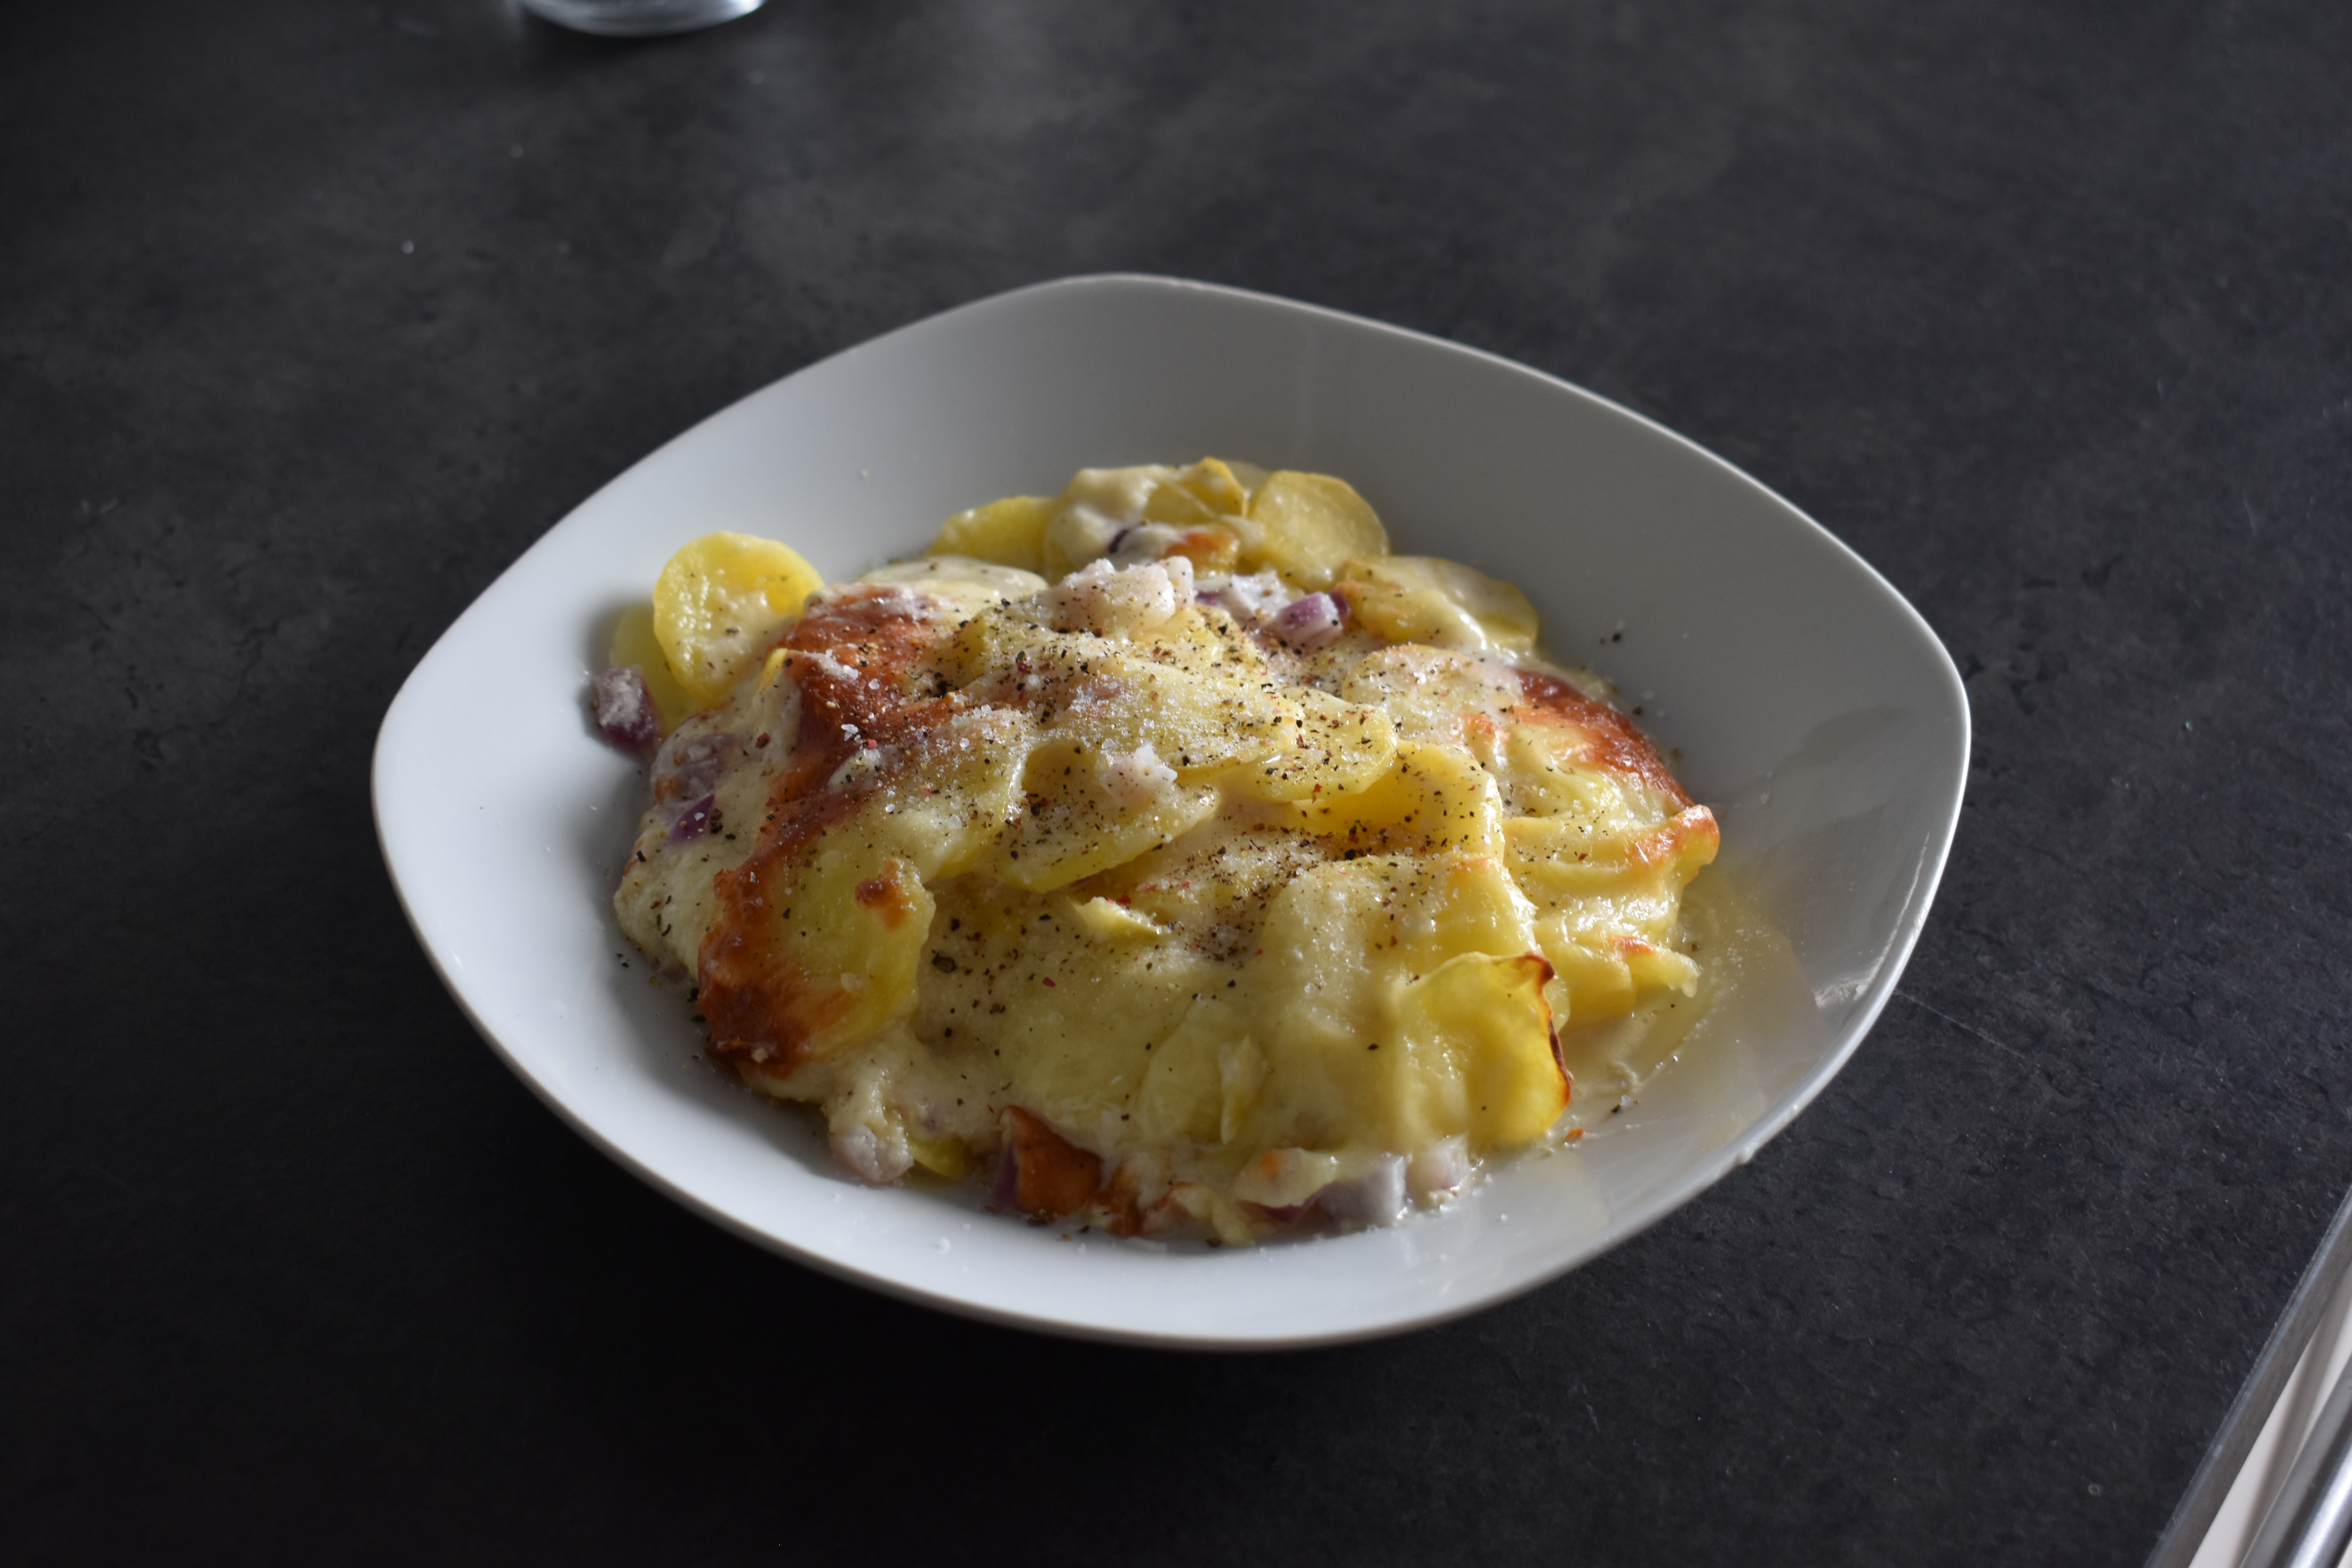
\includegraphics[width=\textwidth]{media/kartoffelgratin.jpg}
\end{figure*}

\begin{wraptable}{r}{0.4\textwidth}
  \centering
  \begin{tabularx}{0.39\textwidth}{|l|X|}
    \toprule
    Menge & Zutaten: \\
    \midrule
    1kg & Kartoffeln \\
    \midrule
    200ml & Sahne \\
    \midrule
    200ml & Milch \\
    \midrule
    2x & Knoblauchzehen \\
    \midrule
    1x & Zwiebel \\
    \midrule
    100g & Käse (z.B. Gruyère oder Emmentaler) \\
    \midrule
    & Salz \\
    \midrule
    & Pfeffer \\
    \midrule
    & Butter \\
    \bottomrule
  \end{tabularx}
\end{wraptable}

Zuerst die Kartoffeln schälen und in dünne Scheiben schneiden. Falls vorhanden, eine Küchenmaschine verwenden. Die Zwiebel und den Knoblauch fein hacken. Den Käse reiben und bereitstellen.

Den Backofen auf 180°C (Ober-/Unterhitze) vorheizen. Eine Auflaufform mit Butter einfetten.

Sahne, Milch, Zwiebeln und Knoblauch in der Auflaufform vermengen und mit Salz und Pfeffer würzen.

Die Kartoffeln in die Auflaufform geben. Den geriebenen Käse gleichmäßig darüber verteilen.

Das Gratin im vorgeheizten Ofen ca. 40–50 Minuten backen, bis die Oberfläche goldbraun ist und die Kartoffeln weich sind. (immer weider mit einem Messer testen, die Dauer hängt von der Dicke der Kartoffelscheiben ab)

\newpage
\end{document}
